\section{Motivations}
\begin{frame}{Motivations}
  \begin{figure}
    \center
    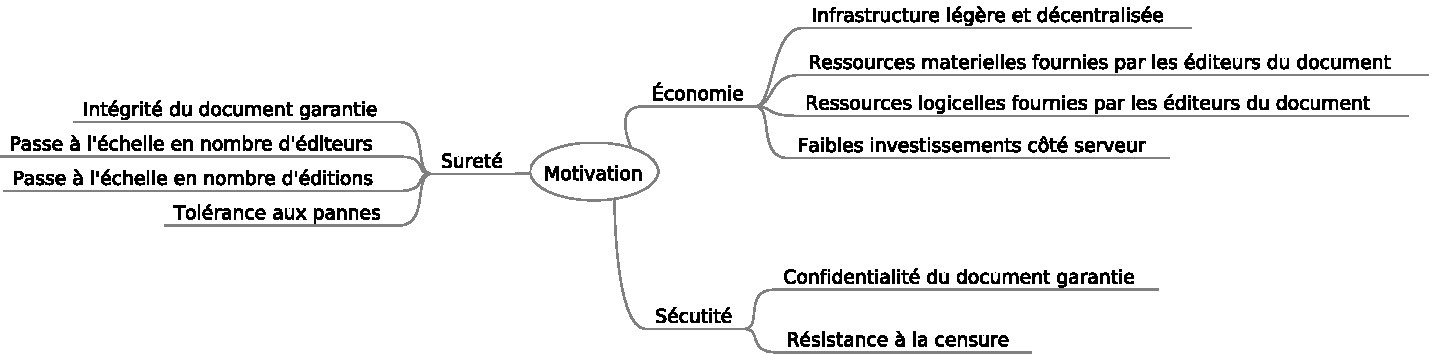
\includegraphics[width=.9\textwidth]{includes/motivations.pdf}
    \caption{Motivations \emph{Mind Map}}
  \end{figure}
\end{frame}
% Voilà ce qu'il en est des motivation économiques, techniques et sociales; mais
% à côté de ça, il y a une autre motivations, c'est que ce projet est également
% une vitrine pour les idées de la recherches puisqu'il utilise à la fois
% l'algorithme du logoot (dire pq) et le langage ciojo (dire pq) qui sont tous
% les deux issues du monde de la recherche. Et donc pour les équipes de
% recherches en charge de ces deux technologies, ce projet peut-être vue comme
% un prototype. Et du coup, se projet à susciter l'interressement à la fois de
% m P. Molli, en charge de l'équie GDD du Lina et initiateur de l'algortihme
% logoot ainsi que monsieur M.Sudholt en charge de l'équipe ASCOLA et du langage
% CRIOJO.
\begin{frame}{Motivations}
  \begin{itemize}
    \item Le projet est une vitrine pour les idées de la recherche
    \item Le projet est un prototype pour les technologies Logoot et Criojo
    \item Le projet suscite l'intéressement des équipes GDD et ASCOLA.
  \end{itemize}
\end{frame}

